\chapterimage{Water1.png} % Chapter heading image

\chapter{Basics of Wastewater Treatment}

\section{Why Treat Wastewater}\index{Why Treat Wastewater}
\begin{itemize}
\item Wastewater is used water from home and industries\\
\item Wastewater must be treated prior to returning it back into the environment - typically into the receiving waters which include lakes, rivers and ocean.


\item Wastewater treatment removes:
\begin{itemize}
\item organic matter
\item inorganic  pollutants including plant nutrients - nitrogen and phosphorous\\
\item pathogenic (disease causing) organisms\\
\end{itemize}

\item Wastewater treatment protects:
\begin{itemize}
\item The environment
\item Human health
\end{itemize}

\item In the receiving waters, inadequately treated wastewater discharge depletes dissolved oxygen levels - \hl{eutrophication}, potentially destructing its normal aquatic life including fish.  Wastewater discharge promotes eutrophication due to:

\begin{itemize}
\item Nutrients such as nitrogen and phosphorous present in wastewater effluent promotes growth of plant and algal matter.  Dissolved oxygen is consumed as a part of the normal decay of this plant and algal matter.  
\item The consumption of organic material present in wastewater discharge by aerobic bacteria also results in oxygen depletion in the receiving waters.  


\end{itemize}
\end{itemize}

\section{Wastewater Treatment Regulations}\index{Wastewater Treatment Regulations}
% \begin{snugshade*}
% \item \noindent\textsc{Wastewater Treatment Regulations}
% \end{snugshade*}

\begin{itemize}
\item The \hl{National Pollutant Discharge Elimination System (NPDES) permit program} was created in 1972 by the Clean Water Act (CWA)
\item Applies to sources that discharge pollutants to waters of the United States.
\item Requires all facilities discharging “pollutants” into any body of water in the USA to obtain and comply with a \hl{NPDES permit}
\item NPDES permit \hl{establishes} \textul{discharge limits}, \textul{monitoring} and \textul{reporting} \hl{requirements}\\
\item The NPDES permitting and enforcement responsibilities have been delegated by the EPA to the State of California for implementation through the \hl{State Water Resources Control Board(SWRCB)} and the \textul{nine} \hl{Regional Water Quality Control Boards (Regional Water Boards)}.
\item In California, NPDES permits are also referred to as waste discharge requirements (WDRs) that regulate discharges to waters of the United States.
\end{itemize}


\section{Wastewater Process Overview}\index{Wastewater Process Overview}
Wastewater treatment involves the following elements:
\subsection{Generation}\index{Generation}
Wastewater originates from domestic, industrial, commercial or agricultural activities. The characteristics of wastewater vary depending on the source. Types of wastewater include: 
\begin{itemize}
\item \hl{Domestic Sewage:}  wastewater derived principally from dwellings, business buildings, institutions, and \\
\item \hl{Industrial Sewage:}  liquid waste from industrial processes\\
\end{itemize}
Typical per person generation of wastewater in the USA is about 70-100 gallons per day

\subsection{Collections}\index{Collections}

\begin{itemize}
\item Wastewater is collected from its point of origin - home, businesses, industries etc. and conveyed via sewer lines to a centralized wastewater treatment facility.  
\item When the rainwater drainage is made part of the sewer system, the system is termed as \hl{Combined System}.  
\item The system where the sewage is conveyed separately from the stormwater flows is termed as \hl{Separated System}.  
\item In the Separated System, the Sanitary Sewers convey the wastewater and the Stormwater Sewer conveys the storm water flows.  
\item For the Combined System, rainstorms pose the threat of overwhelming the sewers and the treatment plant
\end{itemize}


%\begin{figure} 
%
%
%	  	\begin{subfigure}[b]{0.4\linewidth}
%		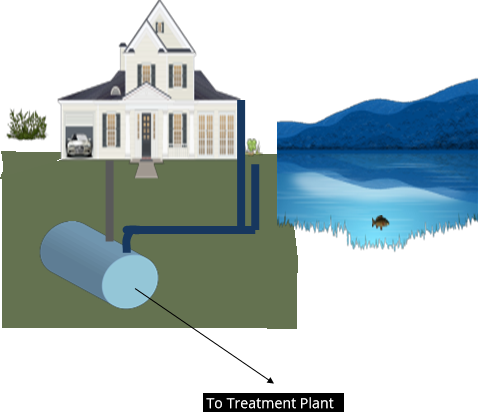
\includegraphics[scale=0.25]{CombinedSystem1} \hspace{0.35cm}
%		\caption{Combined system}
%		\end{subfigure}
%	
%	  	\begin{subfigure}[b]{0.4\linewidth} 
%		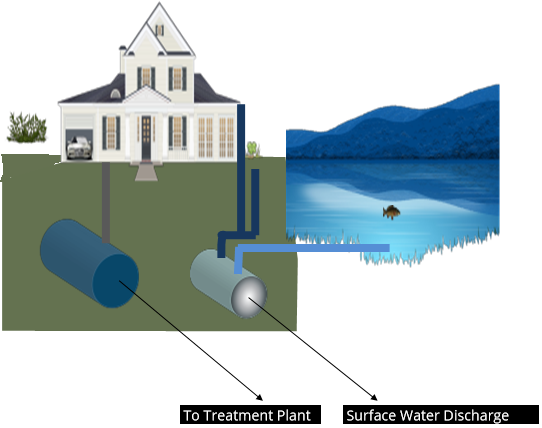
\includegraphics[scale=0.25]{SeperatedSystem1}
%		\caption{Separated systems}
%		\end{subfigure}
%
%
%	\caption{Collections system types}
%
%\end{figure}


	\begin{figure}[h!]
	\centering
  \begin{subfigure}[b]{0.47\linewidth}
  
 \begin{center} 
    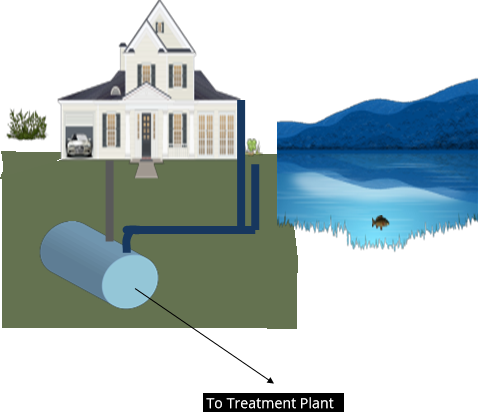
\includegraphics[width=\linewidth]{CombinedSystem1}
    \caption{Combined system}
    \end{center} 
  \end{subfigure}
    \begin{subfigure}[b]{0.50\linewidth}
  \begin{center} 
    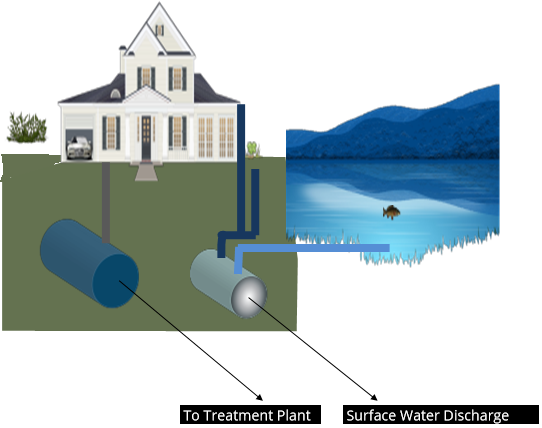
\includegraphics[width=\linewidth]{SeperatedSystem1}
    \caption{Separated systems}
    \end{center} 
  \end{subfigure}
  

  
  \caption{Collections system types}

  \end{figure}



\subsection{Treatment}\index{Treatment}

\begin{itemize}
\item Wastewater treatment includes processes  used for treating the liquid stream and also processes for the treatment of solids which are separated and/or generated during the liquid stream process.
\item The liquid stream wastewater treatment processes involve physical, chemical or biological processes or combinations of these processes depending on the required outflow standards. 
\item Liquid stream is typically treated in a series of steps with increasing level of treatment:
\begin{enumerate}
\item \hl{Preliminary}:  
			
			
		\begin{itemize}
		\item The objective of preliminary treatment is to remove coarse solids and other large materials often found in raw wastewater
		\item Removal of these materials is necessary to enhance the operation and maintenance of subsequent treatment units\\
		\item Preliminary treatment operations typically include a combination of the following processes:
			\begin{itemize}
			\item Screening
			\item Grinding or shredding
			\item Flow measurement
			\item Grit removal
			\item Pre-aeration
			\item Flow equalization
			\end{itemize}
		\end{itemize}
\item \hl{Primary}:
		\begin{itemize}
		\item   The primary process is also a physical process where the separable wastewater solids - solids that float and 			solids that can settle, are removed.
		\item Primary treatment is after preliminary treatment and before secondary treatment
		\item Its two main objectives are: 
			\begin{itemize}
			\item Remove settleable solids
			\item Remove floatable solids
			\end{itemize}
		\item This is a physical process which relies on the physical properties - how heavy or light the suspended solids 				particles are to effect its separation
		\item Provides quiescent conditions for the influent wastewater for the heavier solids to settle and the lighter 				solids to float
		\item Removes settleable solids and floatables
		\item Settled solids are removed as sludge from the bottom of the clarifier
		\item Floatable solids including oil and grease are also removed, as scum from the surface
		\item The shape of the primary clarifier is either rectangular or circular
		\item Effective solids removal in the primary clarifiers will reduce the loading on the expensive secondary treatment 			process.
		\item The amount of solids removed during primary treatment may be enhanced by chemical addition - ferric or ferrous 			chloride as a coagulant and anionic polymer as the flocculant.  This is called Chemically Enhanced Primary Treatment 			(CEPT).
		\end{itemize}
\item \hl{Secondary}:

		\begin{itemize}
		\item While preliminary and primary treatment processes are designed primarily to remove solids from wastewater, 				secondary treatment is for the removal of organics
		\item Secondary treatment is a biological treatment process where microorganisms consume the organic matter present in 			the wastewater.
		\item Secondary treatment involves:
			\begin{itemize}
			\item biological conversion of the dissolved and suspended organics in wastewater into biomass, and
			\item physical settling (separation) process where the solids including the biomass formed during secondary 					treatment is separated and removed from the treated wastewater.
			\end{itemize}
		\item Secondary treatment process incorporates one of the following three approaches:
			\begin{enumerate}
			\item \textbf{Fixed film system}
				\begin{itemize}
				\item Here the microorganisms responsible for the treatment, grow on substrates such
				as rocks, sand or plastic.
				\item When the wastewater is spread over the substrate, the microorganisms up-take the organics present in 						the wastewater
				\item Example of this secondary treatment process include trickling filters and rotating biological 							contactors
				\end{itemize}
			\item \textbf{Suspended Growth System}
				\begin{itemize}
				\item In this type of secondary treatment, the microbes are suspended in the
				wastewater flow being treated. 
				\item Air or oxygen is supplied to maintain an aerobic environment and to keep the microorganisms in 							suspension. 
				\item Example of this secondary treatment approach include the activated sludge treatment process 
				\end{itemize}
			\item \textbf{Pond System}
				\begin{itemize}
				\item Similar to the suspended growth, stabilization ponds are large man made bodies of water which treat 						wastewater using mainly natural processes including sunlight, algae and microorganisms.
				\end{itemize}
			\end{enumerate}
		\end{itemize}


\item \hl{Tertiary or Advanced Treatment:}
	\begin{itemize}
	\item  The tertiary/advanced treatment processes improve the quality of treated water beyond the secondary treatment level. 
	\item  This process may include nutrient removal and disinfection.
	\end{itemize}
	\begin{figure}[h!]
	\centering
\begin{center}
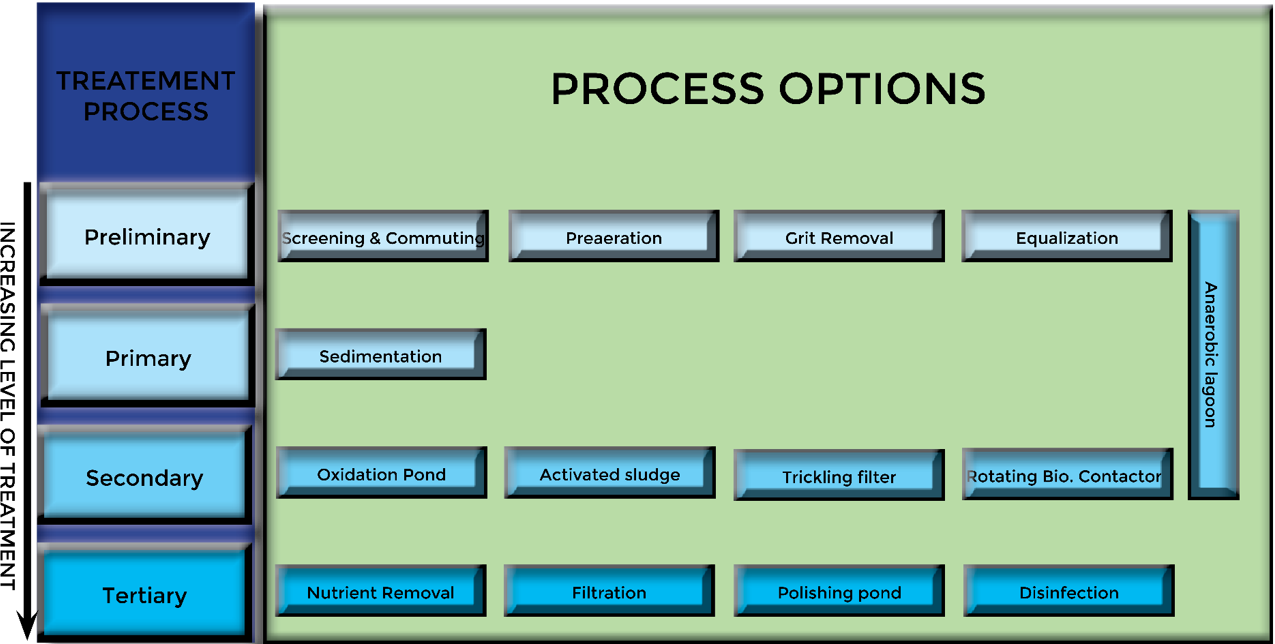
\includegraphics[scale=0.48]{Treatment}
\caption{Process options}
\end{center}
\end{figure}
\end{enumerate}
\vspace{0.5cm}
\item Solids treatment processes are primarily geared to ensure that the solids generated meet the federal regulatory requirements established for wastewater generated solids, at the lowest cost and environmental impact.
\newpage
\textbf{A typical layout/process sequencing in a wastewater treatment plant is shown below:}

	\begin{figure}[h!]
	\centering
\begin{center}
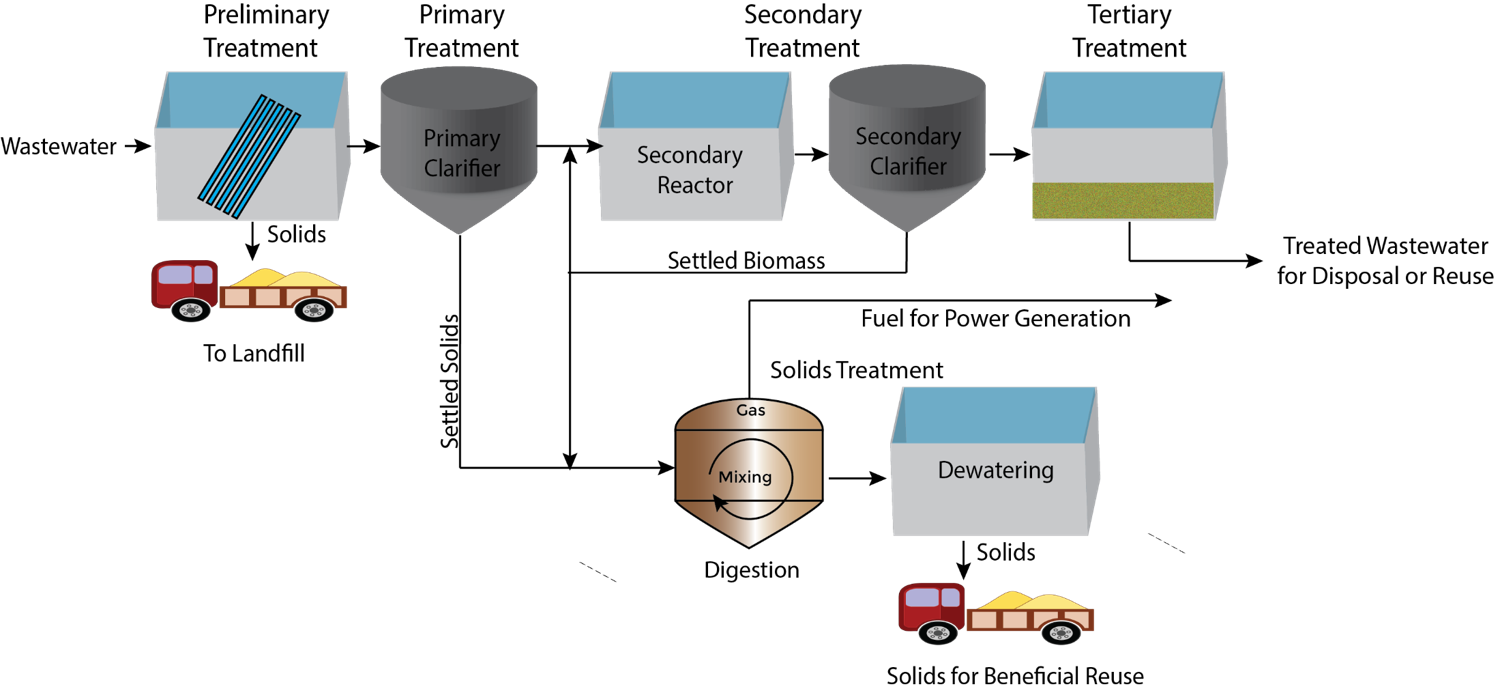
\includegraphics[scale=0.6]{TreatmentFlow}
\end{center}
\caption{Typical wastewater treatment process sequencing}
\end{figure}
\end{itemize}
Individual wastewater treatment processes involve different process options or sequences which are illustrated in Figure 1.3 below:


As the treatment process becomes more advanced along with the increasing awareness of the resources involved in the treatment, there is a move underway to transform Wastewater Treatment Plants (WWTF) to Renewable Resource Recovery Facilities (RRRF) or Water Resource Recovery Facilities (WRRF) - one which produces clean water, recovers energy and generates nutrients.

\subsection{Disposal or Reuse}\index{Disposal or Reuse}

\begin{itemize}
\item Wastewater treatment processes can be designed to \hl{dispose} the treated water where the water is reintroduced to the environment or for \hl{reuse} where the treated water is \hl{reclaimed} or \hl{recycled} - for various purposes including irrigation, industrial use or for potable use.
\item Water disposal methods include:\\
\begin{itemize}
\item \hl{Surface water discharge}
\item \hl{Subsurface discharge}
\end{itemize}
\item Water reuse methods include:\\
\begin{itemize}
\item Potable water reuse
\begin{itemize}
\item \hl{Indirect potable reuse:}  Here the treated water is blended with groundwater or surface water and then reclaimed and treated further 
for drinking (potable) water use
\item \hl{Direct potable reuse:}  Here the treated wastewater is subjected to advanced treatment and introduced directly into a municipal water supply system
\end{itemize}
\item Water reclamation for irrigation or industrial use\\
\item Land application for beneficial use\\
\end{itemize}
\item Solids generated from the wastewater treatment process may be removed and disposed to a landfill or subject to further treatment which may allow for energy recovery - from the organic solids and for beneficial reuse due to its plant nutrient content.\\
\end{itemize}








